\documentclass[12pt]{article}
\usepackage{hyperref}
%\usepackage[super]{natbib}
\usepackage{cite}
\usepackage{graphicx}
\usepackage{caption}
\begin{document}
\title{A Software defined approach for Next generation WLAN networks}
%\section{Abstract}

	
\section{Introduction}
\subsection{WLAN architecture}
\paragraph{}
The IEEE 802.11 standard does not specify the implementation details of an Access Point or a Station. Instead, the IEEE Std 802.11 defines two types of services: the Station Services (SS) and the distribution system services(DS). Due to the lack of implementation details in IEEE Std 802.11 vendors have come up with different architectures and implementations of the WLAN services. Most of the architectures for IEEE Std 802.11 based WLANs can be classified into the following three categories: 

 

    \textbf{Autonomous WLAN Architecture}: In this architecture all IEEE 802.11 services, i.e., the station and distribution services are implemented as part of a single device.  

    \textbf{Centralized WLAN Architecture}: The Centralized WLAN Architecture family typically comprises of a centralized controller (commonly called an Access Controller or AC) and a large number of Base Station devices (wireless nodes, typically called the APs but may not support the complete AP functionality). IEEE 802.11 functions/services are typically not implemented as part of a single device in this architecture but the Base Stations together with the AC support these functions and services. The main function of the Controller (AC) is to manage, control, and configure the access points. Additionally the Controller (AC) may also be an aggregation point for the data plane since it is typically situated in a centralized location in the wireless access network. The AC could be connected to the Base Stations either over an L3 (IP) or L2 (Ethernet) interface. It is possible that multiple ACs are present in a network in order to support redundancy, load balancing, etc. It can also be said that a large percentage of WLAN deployments follow this centralized architecture though the distribution of function/services across the Base Station and the Access Controller may vary. 

    \textbf{Distributed WLAN Architecture}: The third type of WLAN architecture family is a distributed one in which the participating wireless nodes (BSs) form a distributed network among themselves, via wired or wireless media. A wireless mesh network is an example of such an architecture, where the wireless nodes themselves form a mesh network and connect with neighboring wireless nodes over the IEEE 802.11 wireless links. Some of these nodes may also have wired (L2/L3) connections to external networks; such nodes may act as the gateways. 
    

	\subsection{CAPWAP}
	CAPWAP\cite{RFC5416} is the  protocol used in centralized WLAN architecture to manage, control, and configure the access points also called as Wireless Termination Points(WTP). Each vendor uses its own proprietary variant of CAPWAP. CAPWAP can operate in two configurations Split MAC and Local MAC. In Split MAC mode time sensitive functions are placed in AP while non time sensitive functions along with data is tunnelled to the controller via DTLS tunnels. In Local MAC mode all control and management functions are handled locally while data frames are either locally bridged or tunnelled as 802.3 frames to AC. In practice Split MAC mode is used widely over local MAC. 
	
	
    \subsection{Software Defined networking}
    SDN(Software Defined Networking) aims to separate the control plane and the data plane from each other. It enables network devices to be centrally managed, highly programmable and vendor independent.  In case of IEEE 802.11 networks the control plane consists of functions handling control,configuration and management of the STA and AP while data plane as functions handling user data. 
    
    \section{Motivation}
    The thought behind the project was to create a opensource SDN controller for WLAN networks by addressing the following problems:
    \begin{description}
    	\item[$\bullet$ Performance:] SDN philosophy dictates separation of data and control plane. CAPWAP  doesn't follow this as it tunnels all messages including user data to the access controller which introduces unnecessary latency and reduces the data throughput.
    	
    	\item[$\bullet$ Vendor interoperability:] Current wireless controllers in the market only work if the devices they are controlling are from same vendor. This poses a problem in hybrid networks where a entity might wish to use products from different vendors to suit its various needs.
    	 
    	 \item[$\bullet$ Programmability:] Existing wireless products which use the centralized WLAN architecture run on proprietary vendor code. If a network manager wants to perform a specific task on the wireless device it is limited by configuration API provided by the vendor. This translates into a underutilized, unoptimized network.
    \end{description}
    
    
     
    
    \section{Architecture}
\subsection{Control of WLAN Networks}
\subsubsection{Admission control}
In autonomous WLAN architectures association request/response is used to admit a station into the network. In this case the decision to admit is made by AP after checking the capabilities of STA. In case of centralized WLAN architectures this same decision needs to be done at the central controller. Also in centralized case decision to admit a STA can depend on various parameters and not just on capability of STA. Thus we created a new message called admission request which is sent from AP to SDN controller for every new association request. This request contains the STA MAC address and the BSSID on which the association request was received although it may contain many more parameters. For this purpose we modified hostapd\cite{hostapd} to open a tcp socket on the AP and send admission request to the controller. Once controller receives this request it makes a decision whether to admit STA and sends the result using admission reply to the AP.  
\begin{figure}
	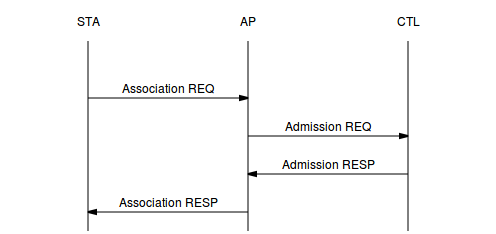
\includegraphics[width=\linewidth]{adm_clf.png}
	\caption{Admission control callflow}
%	\label{fig:boat1}
\end{figure}


\subsubsection{Authentication}
Centralized WLAN architectures widely use 802.1X authentication mechanism for authenticating the STAs. This mechanism is well proven thus we used it without any modifications. For our purposes we used a open source version of a AAA server called FreeRADIUS. The STA acts as  supplicant, AP acts as authenticator while the authenticating server resides on the controller. We used the EAP-PEAP method so that each user would have its own credentials while connecting to a same SSID.\\

\subsubsection{Controller discovery}
In centralized WLAN architectures the AP needs to discover the controller first in order to connect to it. There are several mechanisms to achieve this like providing AP with a IP address or a URL pointing to the controller, use optional fields in DHCP reply etc. We chose to implement the discovery mechanism using a configuration file on AP.
\subsubsection{Quality of service}
In wired networks VLAN tagging is used to enforce QoS. Devices are assigned to VLANs based on different parameters like physical port, device MAC address etc. We implemented the same concept in WLAN using Dynamic VLAN.  In this scheme STAs are assigned different VLANs depending on their credentials. A new sub-interface is created on the AP for every VLAN created. Thus the STAs get quality of service depending on what credentials it uses (e.g guest account will get best effort)


\subsection{Management of WLAN Networks}
   \subsubsection{NETCONF\cite{NETCONF}}
    There are several protocols already developed which may be used to manage and configure Network devices, such as Simple Network Management Protocol (SNMP),TR-069 and NETCONF. After a comparative assessment we feel that NETCONF is the most suitable for WLAN networks as it offers scalability and high level of programmability. NETCONF uses TCP for transport, XML to encode the messages and SSH for security. NETCONF typically consists of a server on the device to be managed and a client on the controller. NETCONF uses YANG\cite{RFC7950} as a data modelling language.\\
    We created a YANG model which allowed us to set default configuration, transmission power and channel for given radio. We also implemented a asynchronous messaging feature of NETCONF called as notifications where the controller gets data when some event is triggered on the device if controller has subscribed for it.
 \section {Simulations}   
 
 
 \section{Testbed}
   \subsection{Hardware}
       \begin{description}
	   	\item[$\bullet$] Mikrotik Routerboard RB433AH 
	   	\item[$\bullet$] Mikrotik Routerboard R52Hn 2.4/5 GHz
	   	\item[$\bullet$] Cisco 2.4/5.8 GHz Omni Antenna
	   	\item[$\bullet$] RF-Element Case
	   	\item[$\bullet$] Toyyo RF Card Stub
	   	
	   	\end{description}
   	 \subsection{Setup}
   	\begin{figure}
   		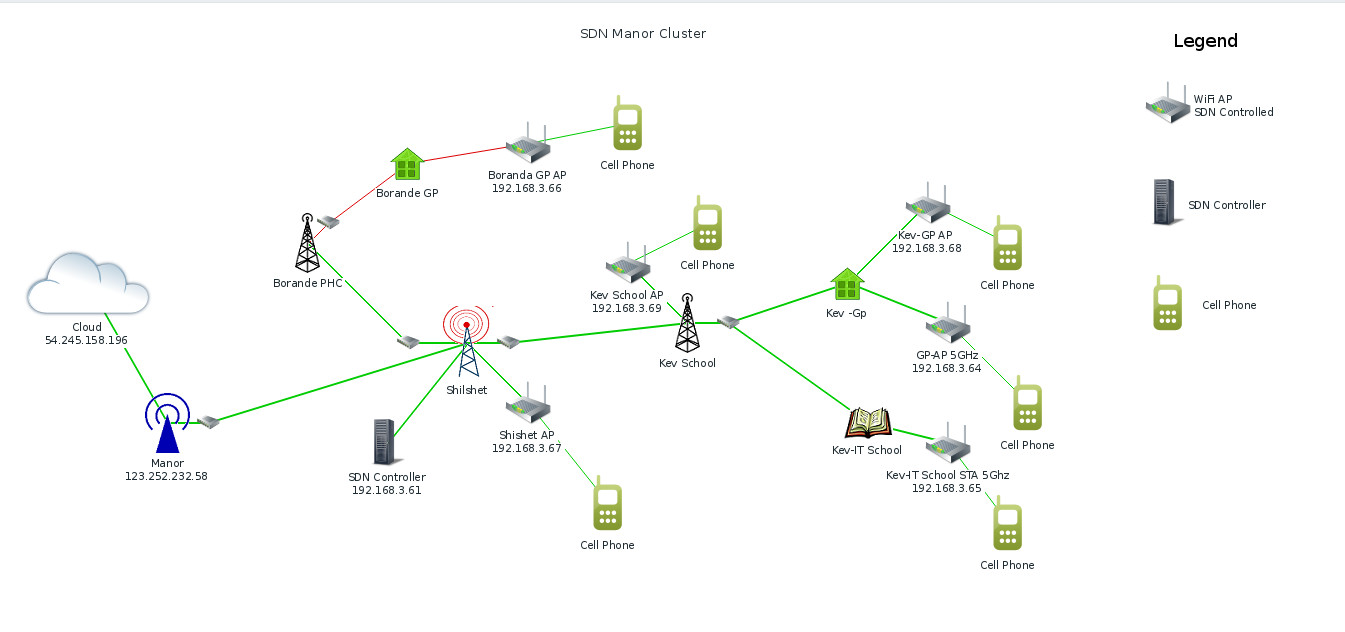
\includegraphics[width=\linewidth]{testbed_setup.jpg}
   		\caption{Testbed topology}
   		\label{fig:boat1}
   	\end{figure}
   	 One of the goals of this project was to provide the internet access in rural unconnected communities, thus we decided to setup our testbed in Palghar district in Maharashtra,India. We deployed wifi APs in 6 different places near Manor. We deployed one AP each in Borande GP, Shilshet GP, Kev School, Kev IT School and two APs in Kev GP. These APs were backhauled using point to point wifi links operating in 5 GHz band. We used zabbix for monitoring the network with a zabbix server running in cloud.
   	 \subsection{Measurements}
   	 
   	 
   	   
   
   %\bibliographystyle{ieeetran}
   %\bibliography{bibref}
    \begin{thebibliography}{1}
    	
    	\bibitem{RFC5416}
    	Myung-Ki Shin, Ki-Hyuk Nam, Hyoung-Jun Kim , "Software-defined networking(SDN): a reference architecture and open APIs" ,\emph{ICTC International Conference}, Oct 2012
    \end{thebibliography}
    
  \end{document}   
